% MeshKit — architecture paper. Build: pdflatex (run twice) or latexmk -pdf.
\documentclass[10pt,twocolumn]{article}

\usepackage[margin=1.9cm,columnsep=0.8cm]{geometry}
\usepackage[T1]{fontenc}
\usepackage[utf8]{inputenc}
\usepackage{lmodern}
\usepackage{microtype}
\usepackage{amsmath}
\usepackage{booktabs}
\usepackage{enumitem}
\usepackage{tikz}
\usetikzlibrary{arrows.meta,positioning,fit,backgrounds,calc,shapes.multipart,chains}
\usepackage{caption}
\captionsetup{font=small,labelfont=bf}
\usepackage[hidelinks]{hyperref}

\newcommand{\meshkit}{\textsc{MeshKit}}
\newcommand{\field}[1]{\texttt{#1}}

% ---- shared TikZ styles -----------------------------------------------------
\tikzset{
  box/.style={draw, rounded corners=2pt, align=center, font=\scriptsize,
              inner sep=4pt, minimum height=6mm},
  app/.style={box, fill=blue!8},
  trust/.style={box, fill=orange!12},
  wire/.style={box, fill=green!10},
  infra/.style={box, fill=gray!12},
  danger/.style={box, fill=red!10},
  lbl/.style={font=\scriptsize\itshape},
  flow/.style={-{Stealth[length=2mm]}, thick},
  dflow/.style={-{Stealth[length=2mm]}, thick, dashed},
  group/.style={draw, rounded corners=3pt, dashed, gray, inner sep=6pt},
}

\title{\meshkit: A Verifiable Trust Layer for App-to-App Agent Transactions\\
\large Architecture and Wire Contract}
\author{Jaegyu Lee\\ \small SeoulTech / MeshKit Project}
\date{August 2026 --- working draft v0.1}

\begin{document}
\maketitle

\begin{abstract}
Mobile platforms are converging on agent-to-app tool registries, yet the
\emph{caller seat} is reserved for the platform's own assistant, and no
deployed protocol lets one app's agent invoke a paid capability of another
app with verifiable user consent. \meshkit{} fills this gap with a small,
frozen wire contract: Ed25519-signed request envelopes and target-signed
receipts that ride as an extension
(\field{ai.meshkit/trust}) on stateless MCP (2026-07-28) tool calls.
The contract is transport-agnostic (HTTP, Android Intents, iOS app-to-app)
and settlement-agnostic (the money leg is a pluggable binding ---
stablecoin rails, x402, or conventional PGs), and is pinned by golden test
vectors that three independent SDKs (Swift, Kotlin, Python) must mutually
verify. This paper gives the architectural overview: the system model, the
canonical wire formats, the fail-closed validation pipeline, the MCP
binding, platform and settlement bindings, and the conformance regime that
makes the contract portable.
\end{abstract}

% ============================================================================
\section{Introduction}

Three observations motivate \meshkit:
\begin{enumerate}[leftmargin=1.4em,itemsep=1pt]
  \item Platform registries (Apple App Intents, Android AppFunctions)
        expose app capabilities to agents, but only the first-party
        assistant may call them --- the \emph{closed caller seat}.
  \item No protocol in deployment performs on-device app-to-app agent
        payments with user-verifiable consent and receipts.
  \item MCP's 2026-07-28 revision made the core stateless: every request
        is self-contained, which is exactly the shape an app-to-app hop
        needs.
\end{enumerate}

\meshkit's thesis is the \emph{open caller}: any authorized agent, not just
the platform assistant, can invoke another app's capability --- provided
every invocation is signed, consented, budgeted, and receipted. The design
principle throughout is that \textbf{trust is carried by the bytes, not by
the channel}: the same signed envelope is valid over HTTP, an Android
Intent, or an iOS app-to-app callback.

Figure~\ref{fig:overview} shows the system at a glance; the rest of the
paper walks down the stack of Figure~\ref{fig:layers}.

% ---------------------------------------------------------------------------
\begin{figure*}[t]
\centering
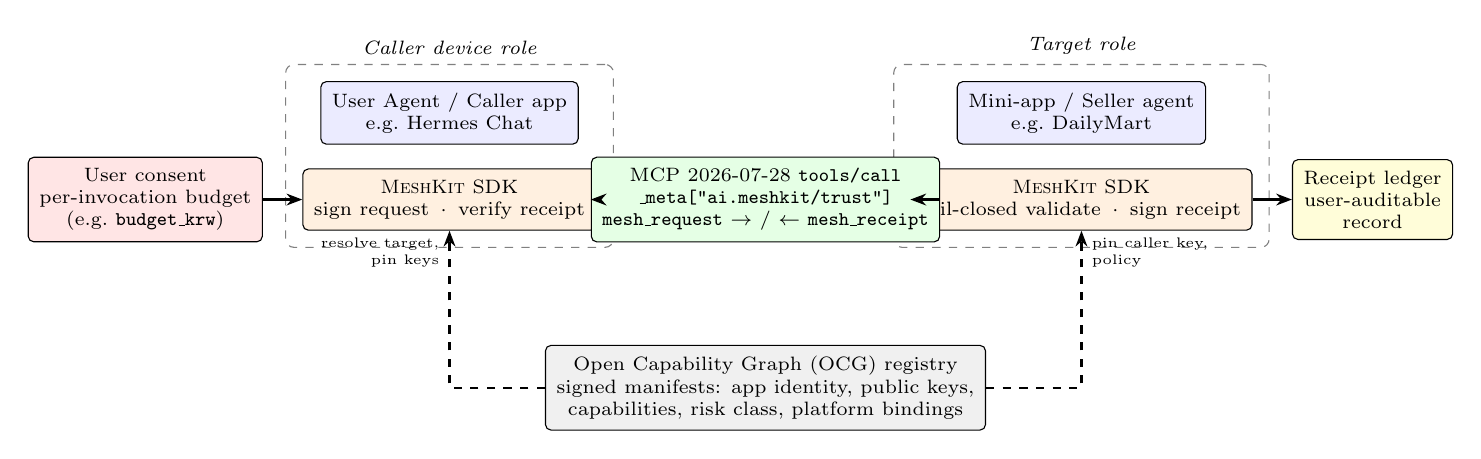
\begin{tikzpicture}[node distance=7mm and 10mm]
  % caller side
  \node[app, minimum width=28mm] (agent) {User Agent / Caller app\\ \scriptsize e.g.\ Hermes Chat};
  \node[trust, below=3mm of agent, minimum width=28mm] (csdk) {\meshkit{} SDK\\ \scriptsize sign request \,$\cdot$\, verify receipt};
  \node[group, fit=(agent)(csdk), label={[lbl]above:{Caller device role}}] (callergrp) {};

  % target side
  \node[app, minimum width=28mm, right=48mm of agent] (mini) {Mini-app / Seller agent\\ \scriptsize e.g.\ DailyMart};
  \node[trust, below=3mm of mini, minimum width=28mm] (tsdk) {\meshkit{} SDK\\ \scriptsize fail-closed validate \,$\cdot$\, sign receipt};
  \node[group, fit=(mini)(tsdk), label={[lbl]above:{Target role}}] (targetgrp) {};

  % wire between
  \node[wire, minimum width=32mm] at ($(csdk)!0.5!(tsdk)$) (mcp)
    {MCP 2026-07-28 \field{tools/call}\\ \scriptsize \field{\_meta["ai.meshkit/trust"]}\\ \scriptsize \field{mesh\_request} $\rightarrow$ / $\leftarrow$ \field{mesh\_receipt}};
  \draw[flow] (csdk) -- (mcp);
  \draw[flow] (mcp) -- (tsdk);

  % registry below
  \node[infra, below=13mm of mcp, minimum width=44mm] (ocg)
    {Open Capability Graph (OCG) registry\\ \scriptsize signed manifests: app identity, public keys,\\ \scriptsize capabilities, risk class, platform bindings};
  \draw[dflow] (ocg.west) -| node[lbl, font=\tiny, pos=0.93, left, align=right]{resolve target,\\ pin keys} (csdk.south);
  \draw[dflow] (ocg.east) -| node[lbl, font=\tiny, pos=0.93, right, align=left]{pin caller key,\\ policy} (tsdk.south);

  % consent + receipts on the sides
  \node[danger, left=5mm of csdk, minimum width=19mm] (consent) {User consent\\ \scriptsize per-invocation budget\\ \scriptsize (e.g.\ \field{budget\_krw})};
  \draw[flow] (consent) -- (csdk);
  \node[box, fill=yellow!15, right=5mm of tsdk, minimum width=19mm] (ledger) {Receipt ledger\\ \scriptsize user-auditable\\ \scriptsize record};
  \draw[flow] (tsdk) -- (ledger);
\end{tikzpicture}
\caption{System overview. A caller app's agent invokes a capability of a
target mini-app. Both sides embed the \meshkit{} SDK; the OCG registry
distributes signed manifests that pin identities and public keys. The only
thing that crosses the wire is a standard MCP tool call carrying the signed
envelope; the only proof of completion is a target-signed receipt.}
\label{fig:overview}
\end{figure*}

% ---------------------------------------------------------------------------
\begin{figure}[t]
\centering
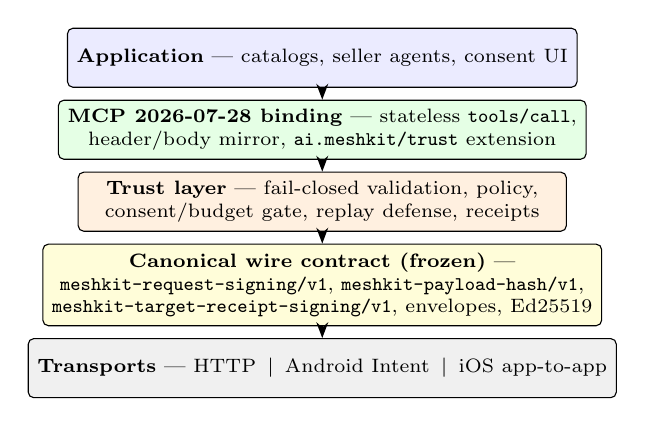
\begin{tikzpicture}[
  layer/.style={draw, rounded corners=2pt, minimum width=62mm, minimum height=7.5mm,
                align=center, font=\scriptsize},
]
  \node[layer, fill=blue!8]   (l4) {\textbf{Application} --- catalogs, seller agents, consent UI};
  \node[layer, fill=green!10, below=1.5mm of l4] (l3)
    {\textbf{MCP 2026-07-28 binding} --- stateless \field{tools/call},\\ header/body mirror, \field{ai.meshkit/trust} extension};
  \node[layer, fill=orange!12, below=1.5mm of l3] (l2)
    {\textbf{Trust layer} --- fail-closed validation, policy,\\ consent/budget gate, replay defense, receipts};
  \node[layer, fill=yellow!15, below=1.5mm of l2] (l1)
    {\textbf{Canonical wire contract (frozen)} ---\\ \field{meshkit-request-signing/v1}, \field{meshkit-payload-hash/v1},\\ \field{meshkit-target-receipt-signing/v1}, envelopes, Ed25519};
  \node[layer, fill=gray!12, below=1.5mm of l1] (l0)
    {\textbf{Transports} --- HTTP \,$\vert$\, Android Intent \,$\vert$\, iOS app-to-app};
  \foreach \a/\b in {l4/l3, l3/l2, l2/l1, l1/l0}
    \draw[flow] (\a) -- (\b);
\end{tikzpicture}
\caption{Layered architecture. Layers 1--2 are identical across all SDKs
and are pinned by golden vectors; layer~0 varies per platform; layer~3 is
the interoperability surface with the MCP ecosystem.}
\label{fig:layers}
\end{figure}

% ============================================================================
\section{System Model and Roles}

\paragraph{Caller.} An app hosting a user-facing agent. It resolves the
target capability from the OCG registry, obtains \emph{user consent with a
budget}, constructs a \field{MeshRequest}, signs it with its registered
Ed25519 request key, and later verifies the receipt.

\paragraph{Target.} An app exposing capabilities (``mini-app'' with an
embedded seller agent). It validates every incoming envelope fail-closed
(\S\ref{sec:pipeline}), executes business logic only after acceptance, and
returns a receipt signed with its registered receipt key.

\paragraph{OCG registry.} A signed, publicly auditable registry of
manifests. A manifest binds: app identity (\field{appId},
\field{bundleId}/package), public keys (\field{publicKeyId}
$\rightarrow$ raw 32-byte Ed25519 key), capability descriptors (id,
version, JSON schema, \emph{risk class} such as \field{spend:money}), and
per-platform bindings (HTTP endpoint, Android action + activity, iOS
scheme). Registration is a Git pull request; CI validates the manifest.

\paragraph{Trust boundaries.} Caller and target trust \emph{only}
(i)~keys pinned via the registry and (ii)~signatures over canonical bytes.
The transport, the OS, and any intermediary superapp router are treated as
untrusted carriers. On Android one extra kernel-verified signal is
admitted: the observed calling package and its signing-certificate hash
(\S\ref{sec:platforms}).

% ============================================================================
\section{Canonical Wire Contract}
\label{sec:wire}

The wire contract is deliberately tiny and \textbf{frozen}: three signing
input formats, one canonicalization rule, one envelope encoding. Any change
requires regenerating the golden vectors and updating all SDKs in the same
commit.

\paragraph{Canonicalization.} A payload (string map) is serialized as
\field{key=value\&key=value\ldots} with keys sorted; every byte of every
key and value that is not an ASCII alphanumeric is percent-encoded in
uppercase hex over its UTF-8 encoding. This gives a unique byte string per
logical payload with no JSON-canonicalization ambiguity.

\paragraph{Nonce-bound payload hash} (\field{meshkit-payload-hash/v1}):
\[
  h = \mathrm{SHA\mbox{-}256}\big(\;
      \field{v1} \,\|\, \field{\textbackslash n} \,\|\,
      \field{nonce=}e(n) \,\|\, \field{\textbackslash n} \,\|\,
      \field{payload=}c(p) \big)
\]
where $e$ is the canonical escape and $c$ the canonical payload form.
Binding the nonce into the hash means a replayed envelope cannot be
re-pointed at a fresh nonce.

\paragraph{Request signing input}
(\field{meshkit-request-signing/v1}): the 12 fields of
Figure~\ref{fig:signing} joined by newlines, signed with Ed25519.
The receipt signing input (\field{meshkit-target-receipt-signing/v1}) is
analogous and additionally \emph{correlates} the receipt to the request
(\field{requestId}, capability id, target identity, and the request's
payload hash), so a receipt can never be detached and re-used for another
transaction.

\paragraph{Envelope.} The signed structure is serialized as sorted-keys
JSON, base64-encoded, and carried as an opaque string
(\field{mesh\_request} / \field{mesh\_receipt}) in whatever slot the
transport offers --- an MCP \field{\_meta} key, an Intent extra, or a query
parameter. Opaqueness is what makes the trust bytes transport-portable.

\begin{figure}[t]
\centering
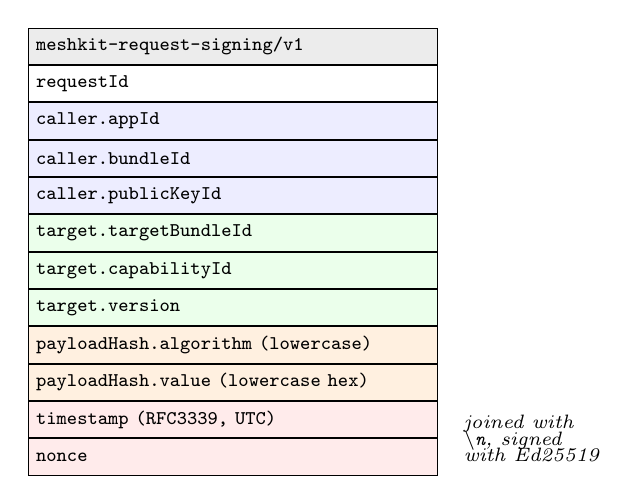
\begin{tikzpicture}[
  f/.style={draw, minimum width=52mm, minimum height=4.6mm, font=\scriptsize\ttfamily,
            align=left, text width=50mm, inner sep=2pt},
  start chain=going below, node distance=0mm
]
  \node[f, on chain, fill=gray!15]  {meshkit-request-signing/v1};
  \node[f, on chain]                {requestId};
  \node[f, on chain, fill=blue!7]   {caller.appId};
  \node[f, on chain, fill=blue!7]   {caller.bundleId};
  \node[f, on chain, fill=blue!7]   {caller.publicKeyId};
  \node[f, on chain, fill=green!8]  {target.targetBundleId};
  \node[f, on chain, fill=green!8]  {target.capabilityId};
  \node[f, on chain, fill=green!8]  {target.version};
  \node[f, on chain, fill=orange!12]{payloadHash.algorithm (lowercase)};
  \node[f, on chain, fill=orange!12]{payloadHash.value (lowercase hex)};
  \node[f, on chain, fill=red!8]    {timestamp (RFC3339, UTC)};
  \node[f, on chain, fill=red!8]    (nonce) {nonce};
  \node[lbl, right=2mm of nonce.north east, anchor=west, align=left]
    {\scriptsize joined with\\[-2pt]\scriptsize \field{\textbackslash n}, signed\\[-2pt]\scriptsize with Ed25519};
\end{tikzpicture}
\caption{The 12-field signing input of
\field{meshkit-request-signing/v1}. Colors: version, request identity,
caller identity (blue), target capability (green), payload commitment
(orange), freshness (red).}
\label{fig:signing}
\end{figure}

% ============================================================================
\section{Trust Layer: Fail-Closed Validation}
\label{sec:pipeline}

The target accepts an invocation only after the ordered pipeline of
Figure~\ref{fig:pipeline} passes \emph{in full}; any failure rejects with a
stable machine-readable code and \textbf{no business logic runs}. Two
ordering decisions matter:

\begin{enumerate}[leftmargin=1.4em,itemsep=1pt]
  \item \emph{Nonce reservation precedes signature verification.} The nonce
        is atomically reserved before the (relatively expensive) signature
        check, so two concurrent copies of the same envelope cannot both
        pass; the loser sees \field{replay\_detected}.
  \item \emph{The consent/budget gate is part of the pipeline, not the
        application.} A \field{spend:money} capability compares
        \field{payload["budget\_krw"]} against the user-approved budget
        inside the trust layer; the application never sees an over-budget
        request (\field{budget\_exceeded}).
\end{enumerate}

\begin{figure}[t]
\centering
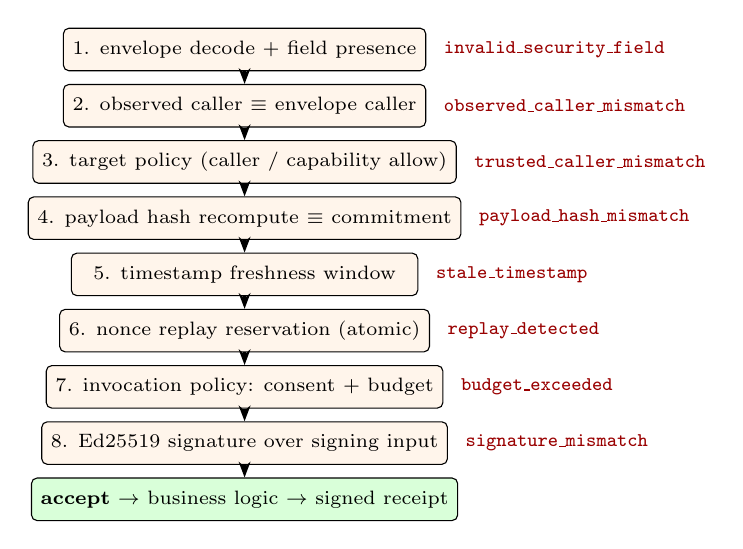
\begin{tikzpicture}[
  s/.style={draw, rounded corners=2pt, minimum width=44mm, minimum height=5.4mm,
            align=center, font=\scriptsize, fill=orange!8},
  r/.style={font=\scriptsize\ttfamily, text=red!60!black, anchor=west},
  start chain=going below, node distance=1.6mm
]
  \node[s, on chain] (s1) {1. envelope decode + field presence};
  \node[s, on chain] (s2) {2. observed caller $\equiv$ envelope caller};
  \node[s, on chain] (s3) {3. target policy (caller / capability allow)};
  \node[s, on chain] (s4) {4. payload hash recompute $\equiv$ commitment};
  \node[s, on chain] (s5) {5. timestamp freshness window};
  \node[s, on chain] (s6) {6. nonce replay reservation (atomic)};
  \node[s, on chain] (s7) {7. invocation policy: consent + budget};
  \node[s, on chain] (s8) {8. Ed25519 signature over signing input};
  \node[s, on chain, fill=green!15] (ok) {\textbf{accept} $\rightarrow$ business logic $\rightarrow$ signed receipt};
  \foreach \a/\b in {s1/s2,s2/s3,s3/s4,s4/s5,s5/s6,s6/s7,s7/s8,s8/ok}
    \draw[flow] (\a) -- (\b);
  \node[r] at ($(s1.east)+(1mm,0)$) {invalid\_security\_field};
  \node[r] at ($(s2.east)+(1mm,0)$) {observed\_caller\_mismatch};
  \node[r] at ($(s3.east)+(1mm,0)$) {trusted\_caller\_mismatch};
  \node[r] at ($(s4.east)+(1mm,0)$) {payload\_hash\_mismatch};
  \node[r] at ($(s5.east)+(1mm,0)$) {stale\_timestamp};
  \node[r] at ($(s6.east)+(1mm,0)$) {replay\_detected};
  \node[r] at ($(s7.east)+(1mm,0)$) {budget\_exceeded};
  \node[r] at ($(s8.east)+(1mm,0)$) {signature\_mismatch};
\end{tikzpicture}
\caption{Fail-closed validation pipeline in the target SDK
(\field{validate\_and\_accept}). Every stage rejects with a stable error
code; business logic is reachable only through stage~8.}
\label{fig:pipeline}
\end{figure}

Completion is symmetric: the caller treats a transaction as done
\emph{only} after verifying a receipt that (a)~is signed by the pinned
target receipt key and (b)~correlates to its own request. A missing,
unsigned, or foreign receipt means the transaction did not happen, whatever
the transport claimed.

% ============================================================================
\section{MCP 2026-07-28 Binding}
\label{sec:mcp}

\meshkit{} maps one OCG capability to one MCP tool and rides the stateless
core of the 2026-07-28 revision (Figure~\ref{fig:seq}):

\begin{itemize}[leftmargin=1.4em,itemsep=1pt]
  \item No handshake or session: discovery is \field{server/discover} /
        \field{tools/list}; every \field{tools/call} is self-contained.
  \item Headers \field{MCP-Protocol-Version}, \field{Mcp-Method},
        \field{Mcp-Name} must mirror the body; the target validates the
        mirror before anything else.
  \item The signed envelope rides in
        \field{params.\_meta["ai.meshkit/trust"].mesh\_request}; the
        target additionally checks
        \emph{envelope payload $\equiv$ tool arguments}, so the argument
        object the model sees is byte-committed by the signature.
  \item The receipt rides in
        \field{result.\_meta["ai.meshkit/trust"].mesh\_receipt}.
  \item Trust failures map to JSON-RPC \field{-32602} with
        \field{error.data.meshkit.code} carrying the pipeline code.
\end{itemize}

Because the extension lives entirely in \field{\_meta}, a
\meshkit-unaware MCP client still sees a well-formed server; a
\meshkit-aware target simply refuses unsigned calls to protected tools.
This is the shape of the planned \field{ai.meshkit/trust} extension
proposal to the MCP extensions registry.

\begin{figure}[t]
\centering
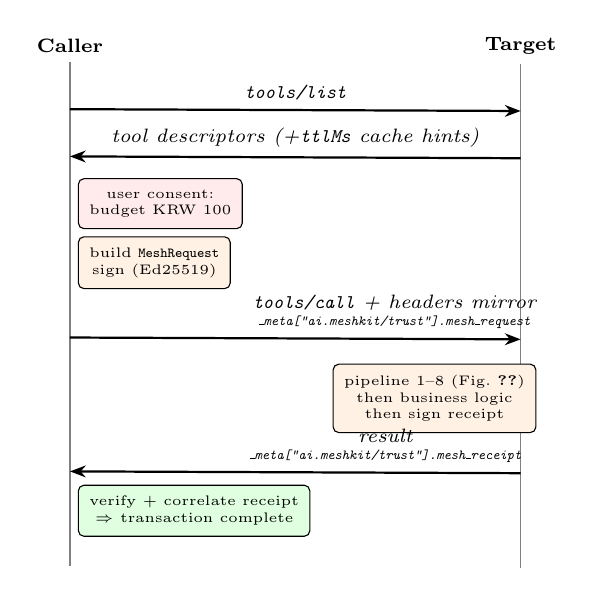
\begin{tikzpicture}[node distance=2mm]
  \node[font=\scriptsize\bfseries] (ct) {Caller};
  \node[font=\scriptsize\bfseries, right=46mm of ct] (tt) {Target};
  \draw[gray] (ct.south) -- ++(0,-6.4cm) coordinate (cb);
  \draw[gray] (tt.south) -- ++(0,-6.4cm) coordinate (tb);
  \newcommand{\msg}[5][0.5]{% [pos] y, from, to, label
    \draw[flow] ($(#3.south)+(0,-#2)$) -- node[lbl, above, align=center, pos=#1]{#5} ($(#4.south)+(0,-#2)$);}
  \msg{0.6cm}{ct}{tt}{\scriptsize\field{tools/list}}
  \msg{1.2cm}{tt}{ct}{\scriptsize tool descriptors (+\field{ttlMs} cache hints)}
  \node[box, fill=red!8, font=\tiny, anchor=west] at ($(ct.south)+(1mm,-1.8cm)$)
    {user consent:\\ budget KRW 100};
  \node[box, fill=orange!10, font=\tiny, anchor=west] at ($(ct.south)+(1mm,-2.55cm)$)
    {build \field{MeshRequest}\\ sign (Ed25519)};
  \msg[0.72]{3.5cm}{ct}{tt}{\scriptsize\field{tools/call} + headers mirror\\[-2pt]
       \tiny\field{\_meta["ai.meshkit/trust"].mesh\_request}}
  \node[box, fill=orange!10, font=\tiny, anchor=east] at ($(tt.south)+(2mm,-4.25cm)$)
    {pipeline 1--8 (Fig.~\ref{fig:pipeline})\\ then business logic\\ then sign receipt};
  \msg[0.3]{5.2cm}{tt}{ct}{\scriptsize result\\[-2pt]
       \tiny\field{\_meta["ai.meshkit/trust"].mesh\_receipt}}
  \node[box, fill=green!12, font=\tiny, anchor=west] at ($(ct.south)+(1mm,-5.7cm)$)
    {verify + correlate receipt\\ $\Rightarrow$ transaction complete};
\end{tikzpicture}
\caption{One signed transaction over stateless MCP. There is no session;
every trust decision is derivable from the single request's bytes.}
\label{fig:seq}
\end{figure}

% ============================================================================
\section{Platform Bindings}
\label{sec:platforms}

The trust bytes are constant; only the carrier changes
(Table~\ref{tab:bindings}).

\begin{table}[t]
\centering\scriptsize
\begin{tabular}{@{}lll@{}}
\toprule
 & \textbf{carrier} & \textbf{caller identity signal} \\
\midrule
HTTP & \field{\_meta} of \field{tools/call} & signature + registry pin only \\
Android & Intent extras \field{mesh\_request} & \field{getCallingPackage()} + \\
 & via \field{startActivityForResult} & signing-cert SHA-256 vs OCG pin \\
iOS & app-to-app envelope in & signature + registry pin only \\
 & query param / callback & \\
\bottomrule
\end{tabular}
\caption{Transport bindings. Android contributes a kernel-verified observed
caller, consumed by pipeline stage~2.}
\label{tab:bindings}
\end{table}

\paragraph{Android specifics.} The intent transport uses action
\field{ai.meshkit.action.INVOKE\_CAPABILITY} with a typed
\field{ActivityResultContract}; keys live in Android Keystore (Ed25519,
API~33+). \field{EXECUTE\_APP\_FUNCTIONS} is privileged
(first-party assistants only), so the Play-legal agent slot is
\field{ROLE\_ASSISTANT}; \meshkit{} additionally enforces an AppFunctions
exposure gate: capabilities with risk \field{spend:money} are \emph{never}
exposed through platform registries, only through the signed path.

% ============================================================================
\section{Settlement Bindings}
\label{sec:settlement}

\meshkit{} deliberately does \emph{not} move money. The trust layer
produces two artifacts --- a user-consented, budget-bounded authorization
(the signed request) and a cryptographically correlated completion claim
(the signed receipt) --- and the actual transfer is delegated to a
\emph{settlement binding}, pluggable in exactly the way transports are
(Figure~\ref{fig:settlement}). A binding contributes one thing to the
frozen contract: a \emph{settlement proof} carried in the receipt's result
map (e.g.\ chain id + transaction hash for an on-chain rail, or a PG
transaction id), which the receipt signature then binds to the original
request. The caller can therefore verify, offline and end-to-end:
\emph{this consent} $\rightarrow$ \emph{this transfer} $\rightarrow$
\emph{this receipt}.

On-chain stablecoin rails are the natural first binding: settlement cost
collapses to network gas, and the protocol itself charges nothing --- there
is no fee-collecting intermediary to fork away. The positioning relative
to adjacent protocols is complementary, not competitive: x402 standardizes
\emph{machine-to-server} payments over HTTP but has no notion of app
identity, user consent, or budget; \meshkit{} supplies precisely that
missing consent layer for \emph{user-authorized app-to-app} spends, and
can settle \emph{through} an x402-style rail. Two invariants hold for
every binding: the core wire contract stays chain- and rail-neutral
(a binding never changes the signing inputs), and the risk-class gates of
\S\ref{sec:pipeline} apply unchanged --- an on-chain leg does not relax
the \field{spend:money} consent and budget requirements.

\begin{figure}[t]
\centering
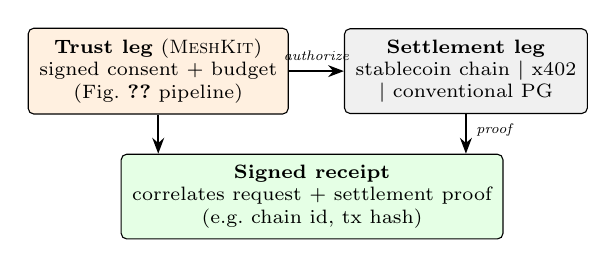
\begin{tikzpicture}[node distance=4mm]
  \node[trust, minimum width=30mm] (auth)
    {\textbf{Trust leg} (\meshkit)\\ \scriptsize signed consent + budget\\ \scriptsize (Fig.~\ref{fig:pipeline} pipeline)};
  \node[infra, right=7mm of auth, minimum width=27mm] (rail)
    {\textbf{Settlement leg}\\ \scriptsize stablecoin chain $\vert$ x402\\ \scriptsize $\vert$ conventional PG};
  \node[wire, below=5mm of $(auth.south)!0.5!(rail.south)$, minimum width=44mm] (rcpt)
    {\textbf{Signed receipt}\\ \scriptsize correlates request $+$ settlement proof\\ \scriptsize (e.g.\ chain id, tx hash)};
  \draw[flow] (auth) -- node[lbl, above]{\tiny authorize} (rail);
  \draw[flow] (auth.south) -- (rcpt.north -| auth.south);
  \draw[flow] (rail.south) -- node[lbl, right, pos=0.4]{\tiny proof} (rcpt.north -| rail.south);
\end{tikzpicture}
\caption{Settlement as a pluggable binding. The trust leg authorizes and
receipts; the settlement leg only transfers. The receipt signature binds
the settlement proof to the original consented request, so verification
never depends on which rail moved the money.}
\label{fig:settlement}
\end{figure}

% ============================================================================
\section{Conformance: The Contract Is a Test}
\label{sec:conformance}

Cross-SDK compatibility is not asserted in prose; it is pinned by
\emph{golden vectors} (fixed seeds, identities, payloads, expected
canonical forms, signing inputs, and hashes) and proven by \emph{mutual
verification} (Figure~\ref{fig:conformance}).

A subtle constraint shapes the regime: Apple CryptoKit's Ed25519 is
\emph{randomized}, not deterministic RFC~8032, so equal signing inputs do
not yield equal signature bytes. Conformance therefore never compares
signatures byte-wise. An implementation is compatible iff:
\begin{enumerate}[leftmargin=1.4em,itemsep=1pt]
  \item its canonical forms, signing inputs, and hashes equal the vectors
        byte-for-byte (\emph{wire level});
  \item every reference SDK verifies its signed envelopes, and it verifies
        theirs (\emph{trust level});
  \item it rejects the full adversarial suite --- tampered payload, replay,
        over-budget, unsigned, imposter caller, stale timestamp
        (\emph{behavioral level}).
\end{enumerate}
The same suite is the course grader: student mini-apps on the SeoulTech
Agentic-AI platform are attacked with exactly these cases, so every
passing team is, by construction, a new conforming implementation.

\begin{figure}[t]
\centering
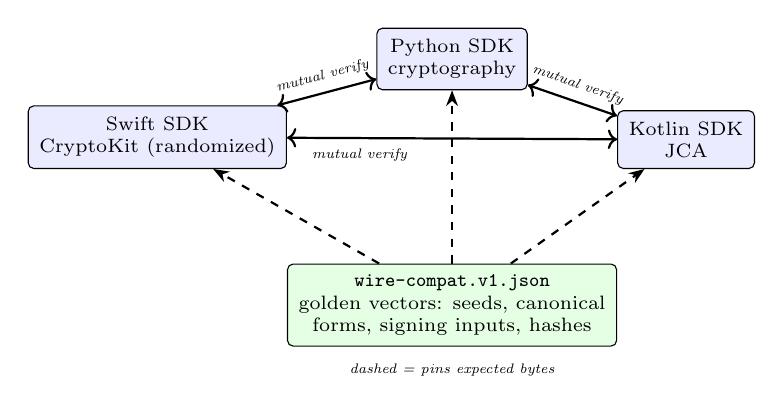
\begin{tikzpicture}
  \node[wire, minimum width=34mm] (vec)
    {\field{wire-compat.v1.json}\\ \scriptsize golden vectors: seeds, canonical\\ \scriptsize forms, signing inputs, hashes};
  \node[app, above left=12mm and 0mm of vec] (swift) {Swift SDK\\ \scriptsize CryptoKit (randomized)};
  \node[app, above right=12mm and 0mm of vec] (kotlin) {Kotlin SDK\\ \scriptsize JCA};
  \node[app, above=22mm of vec] (py) {Python SDK\\ \scriptsize cryptography};
  \foreach \x in {swift,kotlin,py}
    \draw[dflow] (vec) -- (\x);
  \draw[flow, <->] (swift) -- node[lbl, above, sloped]{\tiny mutual verify} (py);
  \draw[flow, <->] (py) -- node[lbl, above, sloped]{\tiny mutual verify} (kotlin);
  \draw[flow, <->] (swift) -- node[lbl, below, pos=0.22]{\tiny mutual verify} (kotlin);
  \node[lbl, below=1mm of vec] {\tiny dashed = pins expected bytes};
\end{tikzpicture}
\caption{Conformance triangle. Vectors pin every intermediate byte;
signatures are proven by cross-verification, never byte equality, because
CryptoKit signatures are randomized.}
\label{fig:conformance}
\end{figure}

% ============================================================================
\section{Ecosystem and Roadmap}

Figure~\ref{fig:ecosystem} places the components in their delivery
context. The open-source launch runs four workstreams: (WS1) a
\field{meshkit-conformance} package making the vectors + attack suite the
public certification path; (WS2) seven specification documents (canonical
form, request, receipt, trust extension, registry, transport bindings,
settlement bindings);
(WS3) governance (DCO, wire-freeze rule, security policy); (WS4) the
\field{ai.meshkit/trust} extension proposal to the MCP registry, gated on
public launch plus first-cohort evidence. The course cohort doubles as the
empirical demonstration of the open-caller thesis: dozens of independent,
mutually-untrusting teams transacting through signed envelopes.

\begin{figure}[t]
\centering
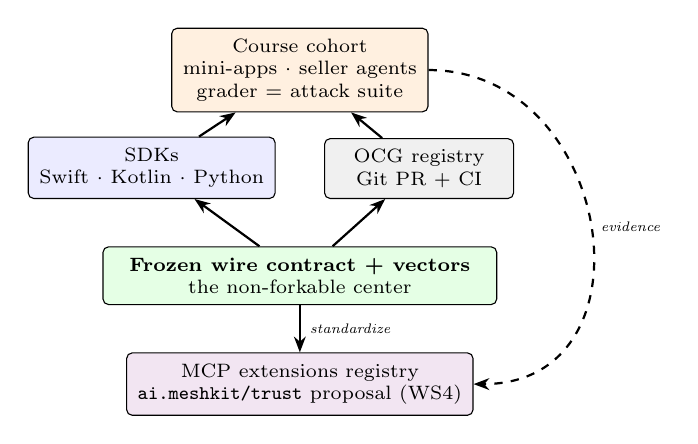
\begin{tikzpicture}[node distance=3mm]
  \node[wire, minimum width=50mm] (core)
    {\textbf{Frozen wire contract + vectors}\\ \scriptsize the non-forkable center};
  \node[app, above left=6mm and -22mm of core, minimum width=24mm] (sdks)
    {SDKs\\ \scriptsize Swift $\cdot$ Kotlin $\cdot$ Python};
  \node[infra, above right=6mm and -22mm of core, minimum width=24mm] (reg)
    {OCG registry\\ \scriptsize Git PR + CI};
  \node[trust, above=17mm of core, minimum width=30mm] (course)
    {Course cohort\\ \scriptsize mini-apps $\cdot$ seller agents\\ \scriptsize grader = attack suite};
  \node[box, fill=violet!10, below=6mm of core, minimum width=42mm] (mcpreg)
    {MCP extensions registry\\ \scriptsize \field{ai.meshkit/trust} proposal (WS4)};
  \draw[flow] (core) -- (sdks);
  \draw[flow] (core) -- (reg);
  \draw[flow] (sdks) -- (course);
  \draw[flow] (reg) -- (course);
  \draw[dflow] (course.east) to[out=0, in=0, looseness=1.5]
    node[lbl, right, pos=0.5]{\tiny evidence} (mcpreg.east);
  \draw[flow] (core) -- node[lbl, right]{\tiny standardize} (mcpreg);
\end{tikzpicture}
\caption{Delivery ecosystem. The frozen contract feeds the SDKs and
registry; the course cohort exercises them at scale and produces the
evidence backing the MCP extension proposal.}
\label{fig:ecosystem}
\end{figure}

% ============================================================================
\section{Conclusion}

\meshkit{} shows that app-to-app agent transactions need surprisingly
little new machinery: a canonical byte form, two Ed25519 signing inputs,
a nonce-bound hash, and an ordered fail-closed pipeline --- all riding as
one \field{\_meta} extension on stateless MCP. The layer that authorizes
and receipts is deliberately separated from the layers that carry and
settle: transports and settlement rails (including on-chain stablecoin
legs at gas-only cost) plug in beneath an unchanged contract. Freezing
that contract in executable vectors is what makes the rest --- three SDKs,
three transports, pluggable settlement, a classroom of independent
implementations, and a path to standardization --- composable rather than
aspirational.

\end{document}
